\subsection{Login and Registration}
\subsubsection{Class Diagram}

\begin{figure}[H]
    \centering
    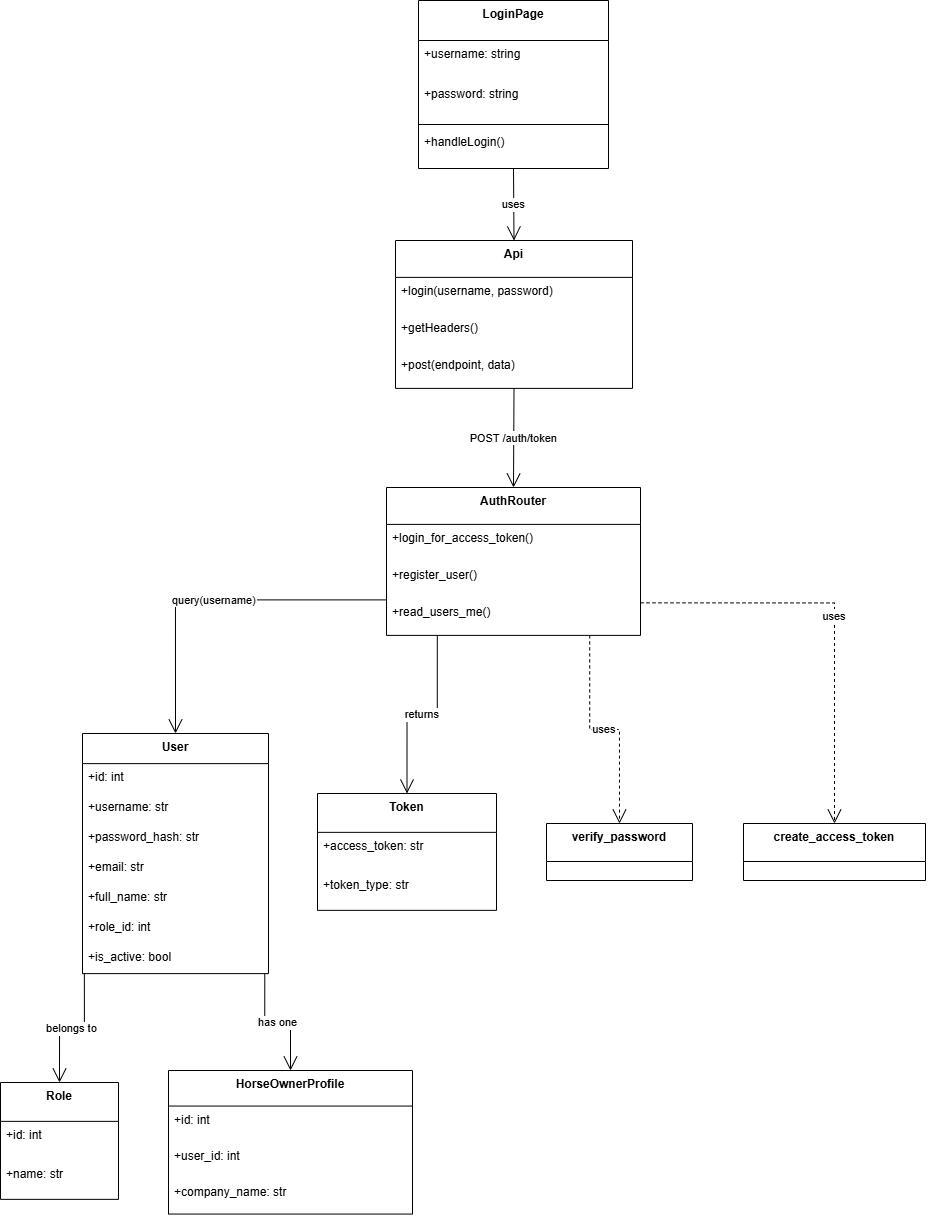
\includegraphics[width=\textwidth,height=0.78\textheight,keepaspectratio]{figures/design/horse_owner/login_class_diagram.png}
    \caption{Login Class Diagram}
    \label{fig:horse_owner_login_class_diagram}
\end{figure}

\subsubsection{Sequence Diagram}

\begin{figure}[H]
    \centering
    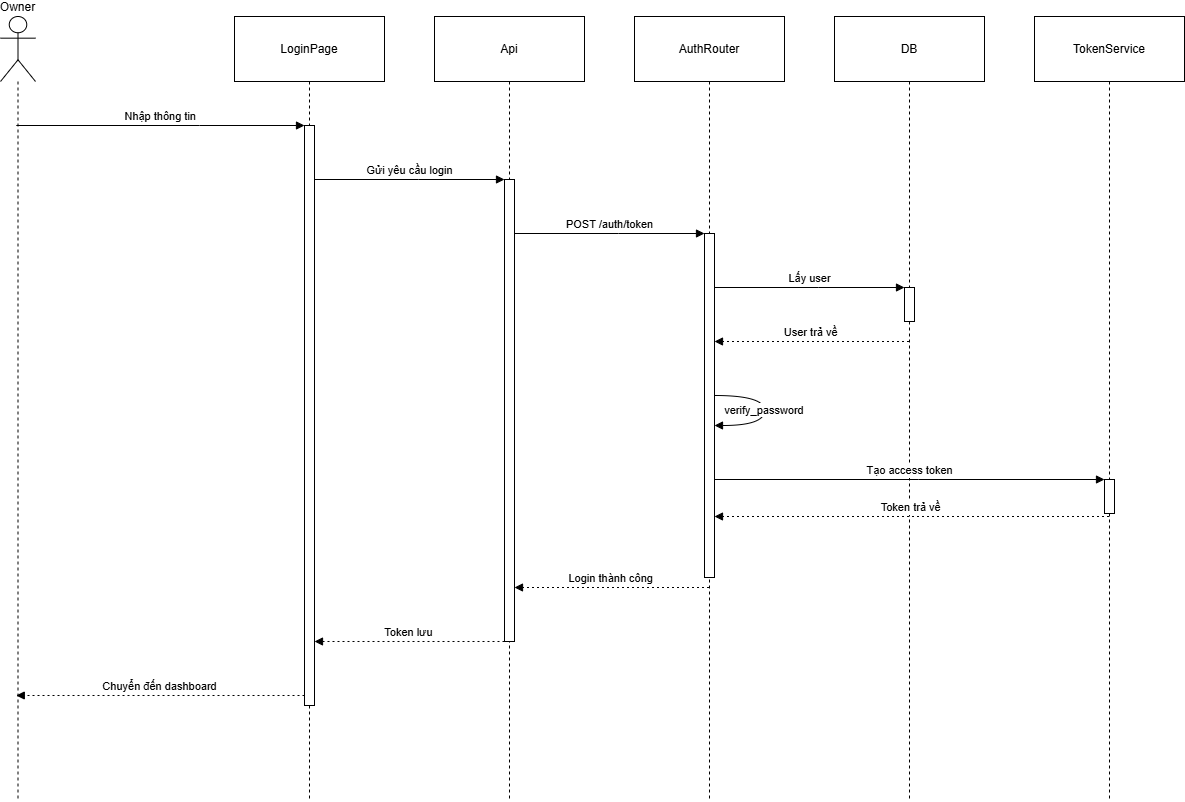
\includegraphics[width=\textwidth,height=0.78\textheight,keepaspectratio]{figures/design/horse_owner/login_sequence_diagram.png}
    \caption{Login Sequence Diagram}
    \label{fig:horse_owner_login_sequence_diagram}
\end{figure}


\subsubsection{Class Specification}

\begingroup
\small
\setlength{\tabcolsep}{3pt}
\begin{longtable}{|>{\raggedright\arraybackslash}p{0.15\textwidth}|>{\raggedright\arraybackslash}p{0.31\textwidth}|>{\raggedright\arraybackslash}p{0.14\textwidth}|>{\raggedright\arraybackslash}p{0.25\textwidth}|}
\caption{Login class specification}
\label{tab:horse_owner_login_class_spec} \\
\hline
\tableHeader
\textbf{Class} & \textbf{Attributes / Methods} & \textbf{Type} & \textbf{Description} \\
\hline
\endfirsthead
\hline
\tableHeader
\textbf{Class} & \textbf{Attributes / Methods} & \textbf{Type} & \textbf{Description} \\
\hline
\endhead
LoginPage & username, password, handleLogin() & state / action & UI component that collects login credentials and calls the API. \\
\hline
Api & login(), post(), getHeaders() & service / helper & Calls \texttt{POST /auth/token}, stores JWT, and prepares request headers. \\
\hline
AuthRouter & login\_for\_access\_token(), read\_users\_me() & controller / route & Validates username/password and issues bearer tokens. \\
\hline
User & id, username, password\_hash, email, full\_name, role\_id, is\_active & entity & Database entity representing an application user. \\
\hline
Role & id, name & entity & Defines user roles, including \texttt{OWNER}. \\
\hline
Token & access\_token, token\_type & DTO & Response payload returned after successful login. \\
\hline
HorseOwner\allowbreak{}Profile & id, user\_id, company\_name & entity & Owner-specific profile linked to the User entity. \\
\hline
\end{longtable}
\endgroup

\subsection{Horse Owner Authentication and Authorization}
\subsubsection{Class Diagram}

\begin{figure}[H]
    \centering
    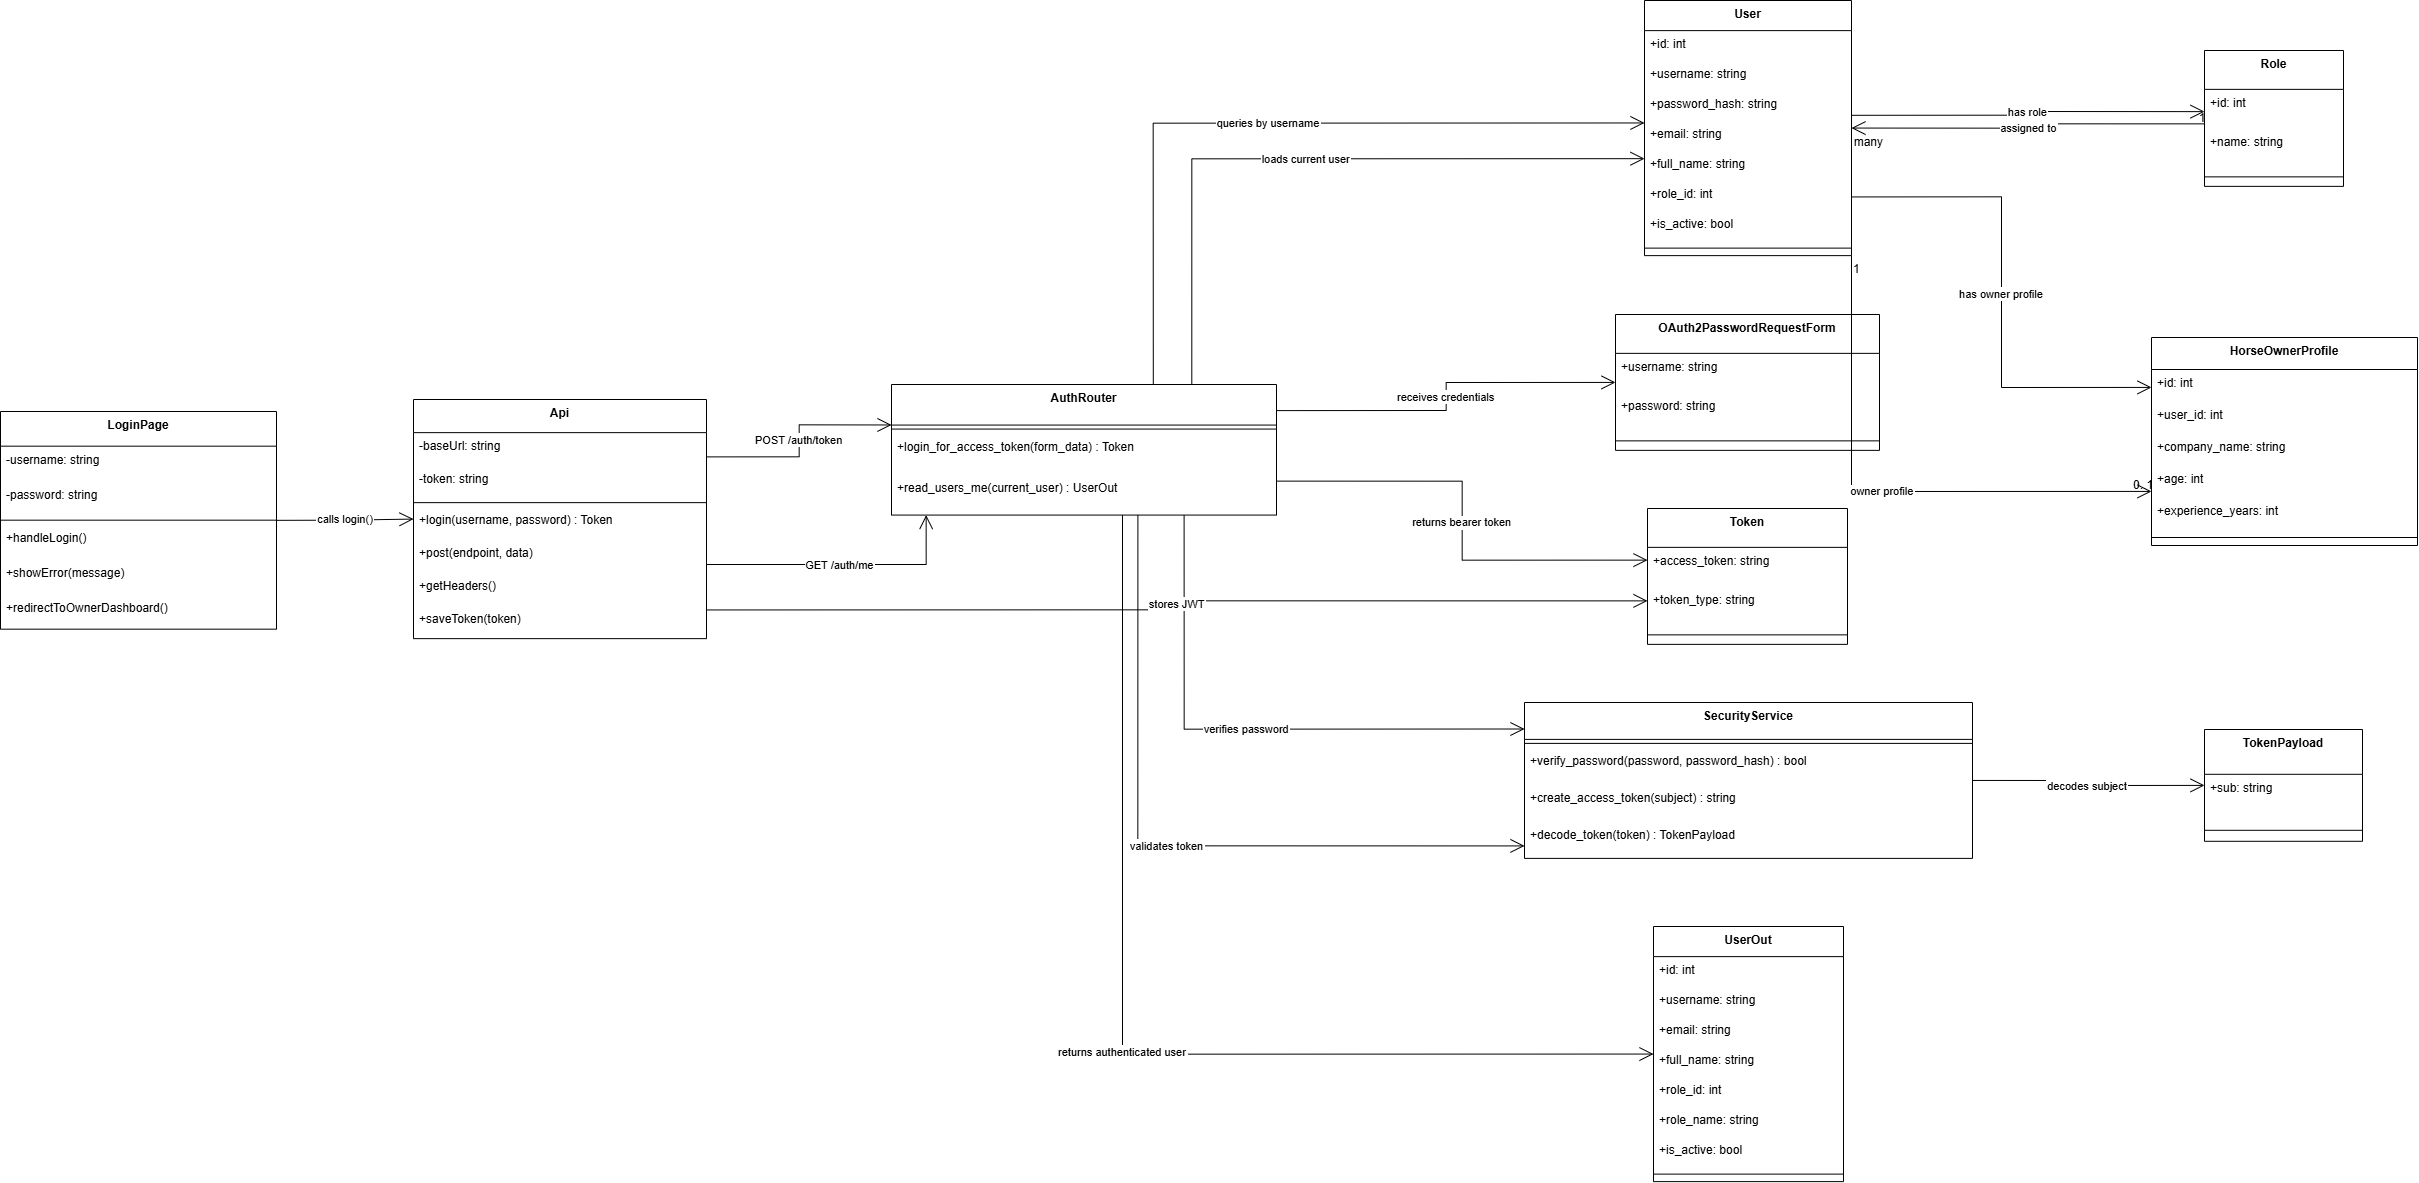
\includegraphics[width=\textwidth,height=0.78\textheight,keepaspectratio]{figures/design/horse_owner/authentication_class_diagram.png}
    \caption{Horse Owner Authentication and Authorization Class Diagram}
    \label{fig:horse_owner_authentication_class_diagram}
\end{figure}

\subsubsection{Sequence Diagram}

\begin{figure}[H]
    \centering
    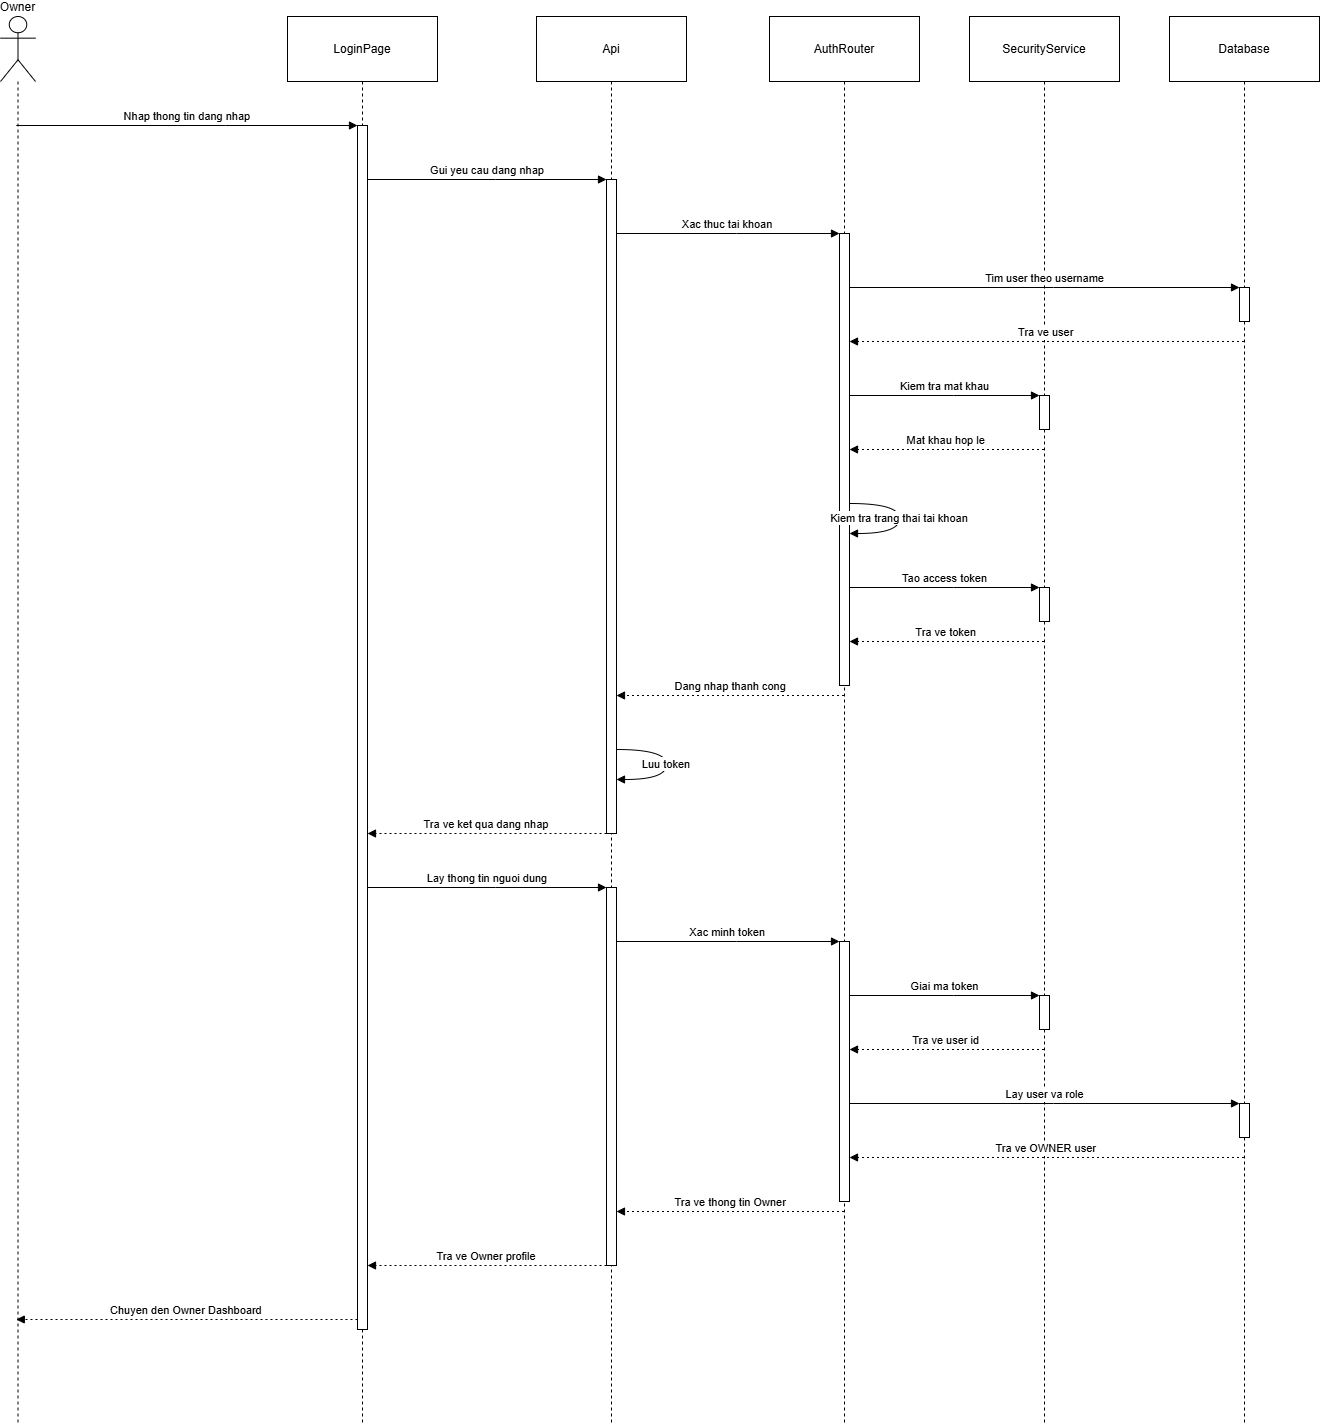
\includegraphics[width=\textwidth,height=0.78\textheight,keepaspectratio]{figures/design/horse_owner/authentication_sequence_diagram.png}
    \caption{Horse Owner Authentication and Authorization Sequence Diagram}
    \label{fig:horse_owner_authentication_sequence_diagram}
\end{figure}


\subsubsection{Class Specification}

\begingroup
\small
\setlength{\tabcolsep}{3pt}
\begin{longtable}{|>{\raggedright\arraybackslash}p{0.16\textwidth}|>{\raggedright\arraybackslash}p{0.30\textwidth}|>{\raggedright\arraybackslash}p{0.14\textwidth}|>{\raggedright\arraybackslash}p{0.25\textwidth}|}
\caption{Horse Owner authentication and authorization class specification}
\label{tab:horse_owner_authentication_class_spec} \\
\hline
\tableHeader
\textbf{Class} & \textbf{Attributes / Methods} & \textbf{Type} & \textbf{Description} \\
\hline
\endfirsthead
\hline
\tableHeader
\textbf{Class} & \textbf{Attributes / Methods} & \textbf{Type} & \textbf{Description} \\
\hline
\endhead
LoginPage & username, password, handleLogin(), showError(), redirectToOwnerDashboard() & boundary / UI & Collects owner credentials, sends the login request, displays authentication errors, and redirects a valid owner to the owner dashboard. \\
\hline
Api & baseUrl, token, login(), post(), getHeaders(), saveToken() & service / helper & Sends authentication requests to the backend, stores the JWT token, and prepares authorization headers for protected owner operations. \\
\hline
AuthRouter & login\_for\_access\_token(), read\_users\_me() & controller / route & Processes login requests, validates submitted credentials, issues bearer tokens, and returns authenticated user information. \\
\hline
Security\allowbreak{}Service & verify\_password(), create\_access\_token(), decode\_token() & service & Verifies password hashes and creates or validates JWT tokens used in the owner authentication flow. \\
\hline
OAuth2Password\allowbreak{}RequestForm & username, password & DTO / request & Carries the submitted username and password from the login form to the authentication endpoint. \\
\hline
Token & access\_token, token\_type & DTO / response & Represents the bearer token returned to the frontend after successful authentication. \\
\hline
Token\allowbreak{}Payload & sub & DTO / payload & Stores the user identifier decoded from the JWT token when resolving the current authenticated user. \\
\hline
User & id, username, password\_hash, email, full\_name, role\_id, is\_active & entity & Stores account and credential information used to authenticate the owner and verify account status. \\
\hline
Role & id, name & entity & Defines user roles and allows the system to confirm that the authenticated account has the \texttt{OWNER} role. \\
\hline
HorseOwner\allowbreak{}Profile & id, user\_id, company\_name, age, experience\_years & entity & Stores owner-specific profile information linked to the authenticated user account. \\
\hline
UserOut & id, username, email, full\_name, role\_id, role\_name, is\_active & DTO / response & Returns authenticated user details to the frontend so the dashboard can render owner-specific screens. \\
\hline
\end{longtable}
\endgroup

\subsection{Horse Owner Management Operations}
\subsubsection{Class Diagram}

\begin{figure}[H]
    \centering
    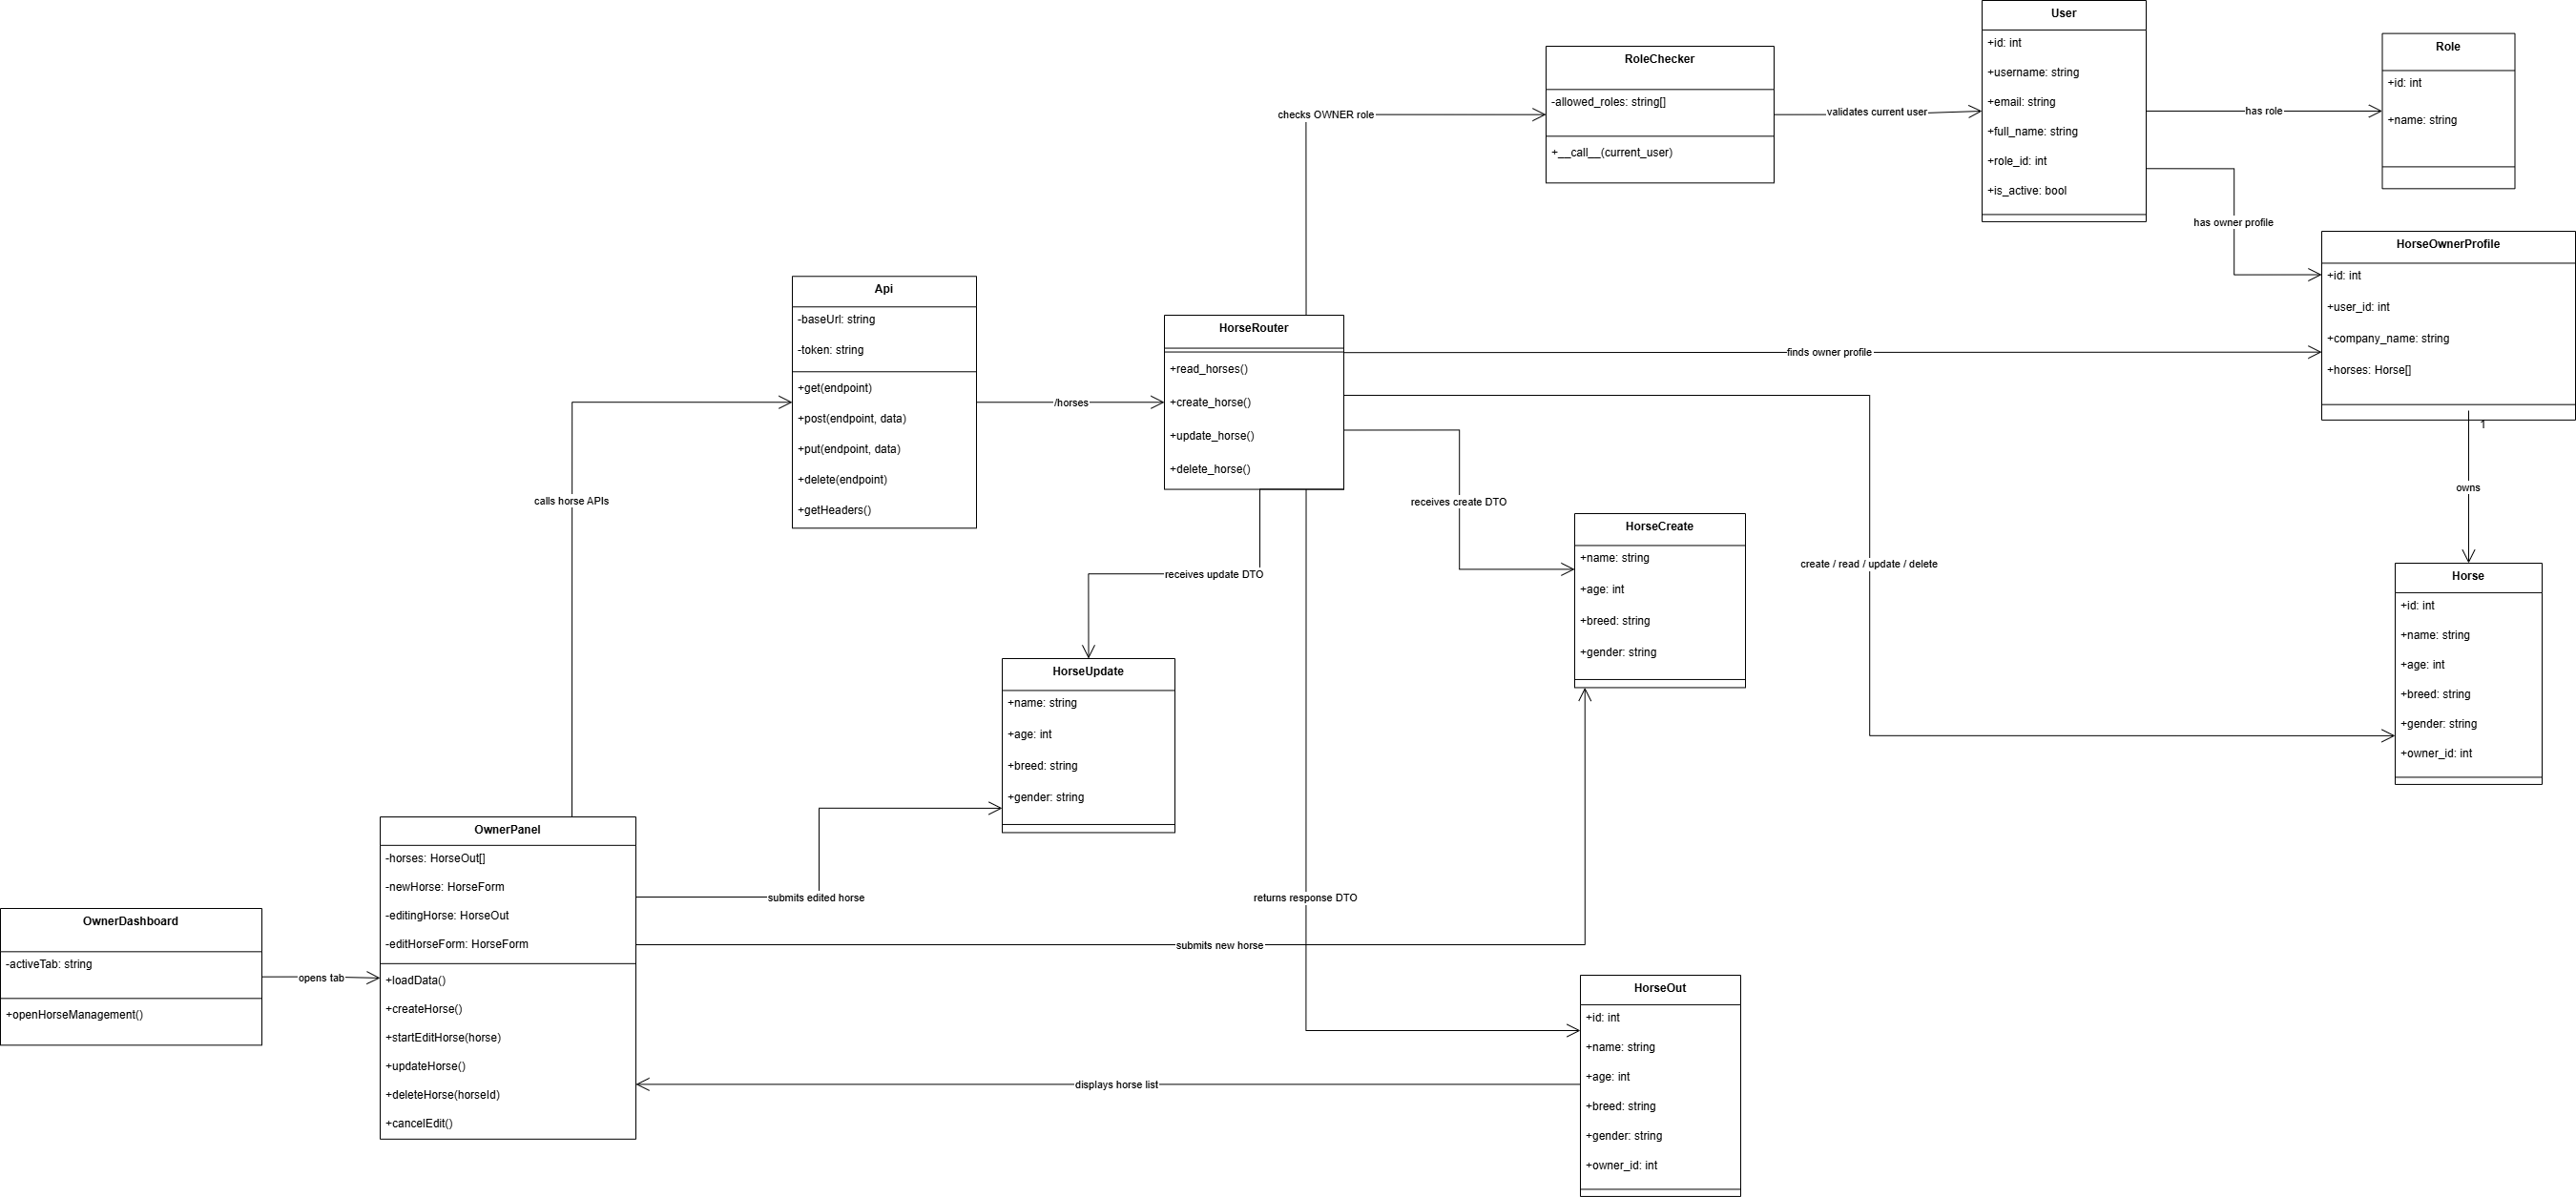
\includegraphics[width=\textwidth,height=0.78\textheight,keepaspectratio]{figures/design/horse_owner/management_class.png}
    \caption{Horse Owner Management Operations Class Diagram}
    \label{fig:horse_owner_management_class_diagram}
\end{figure}

\subsubsection{Sequence Diagram}

\begin{figure}[H]
    \centering
    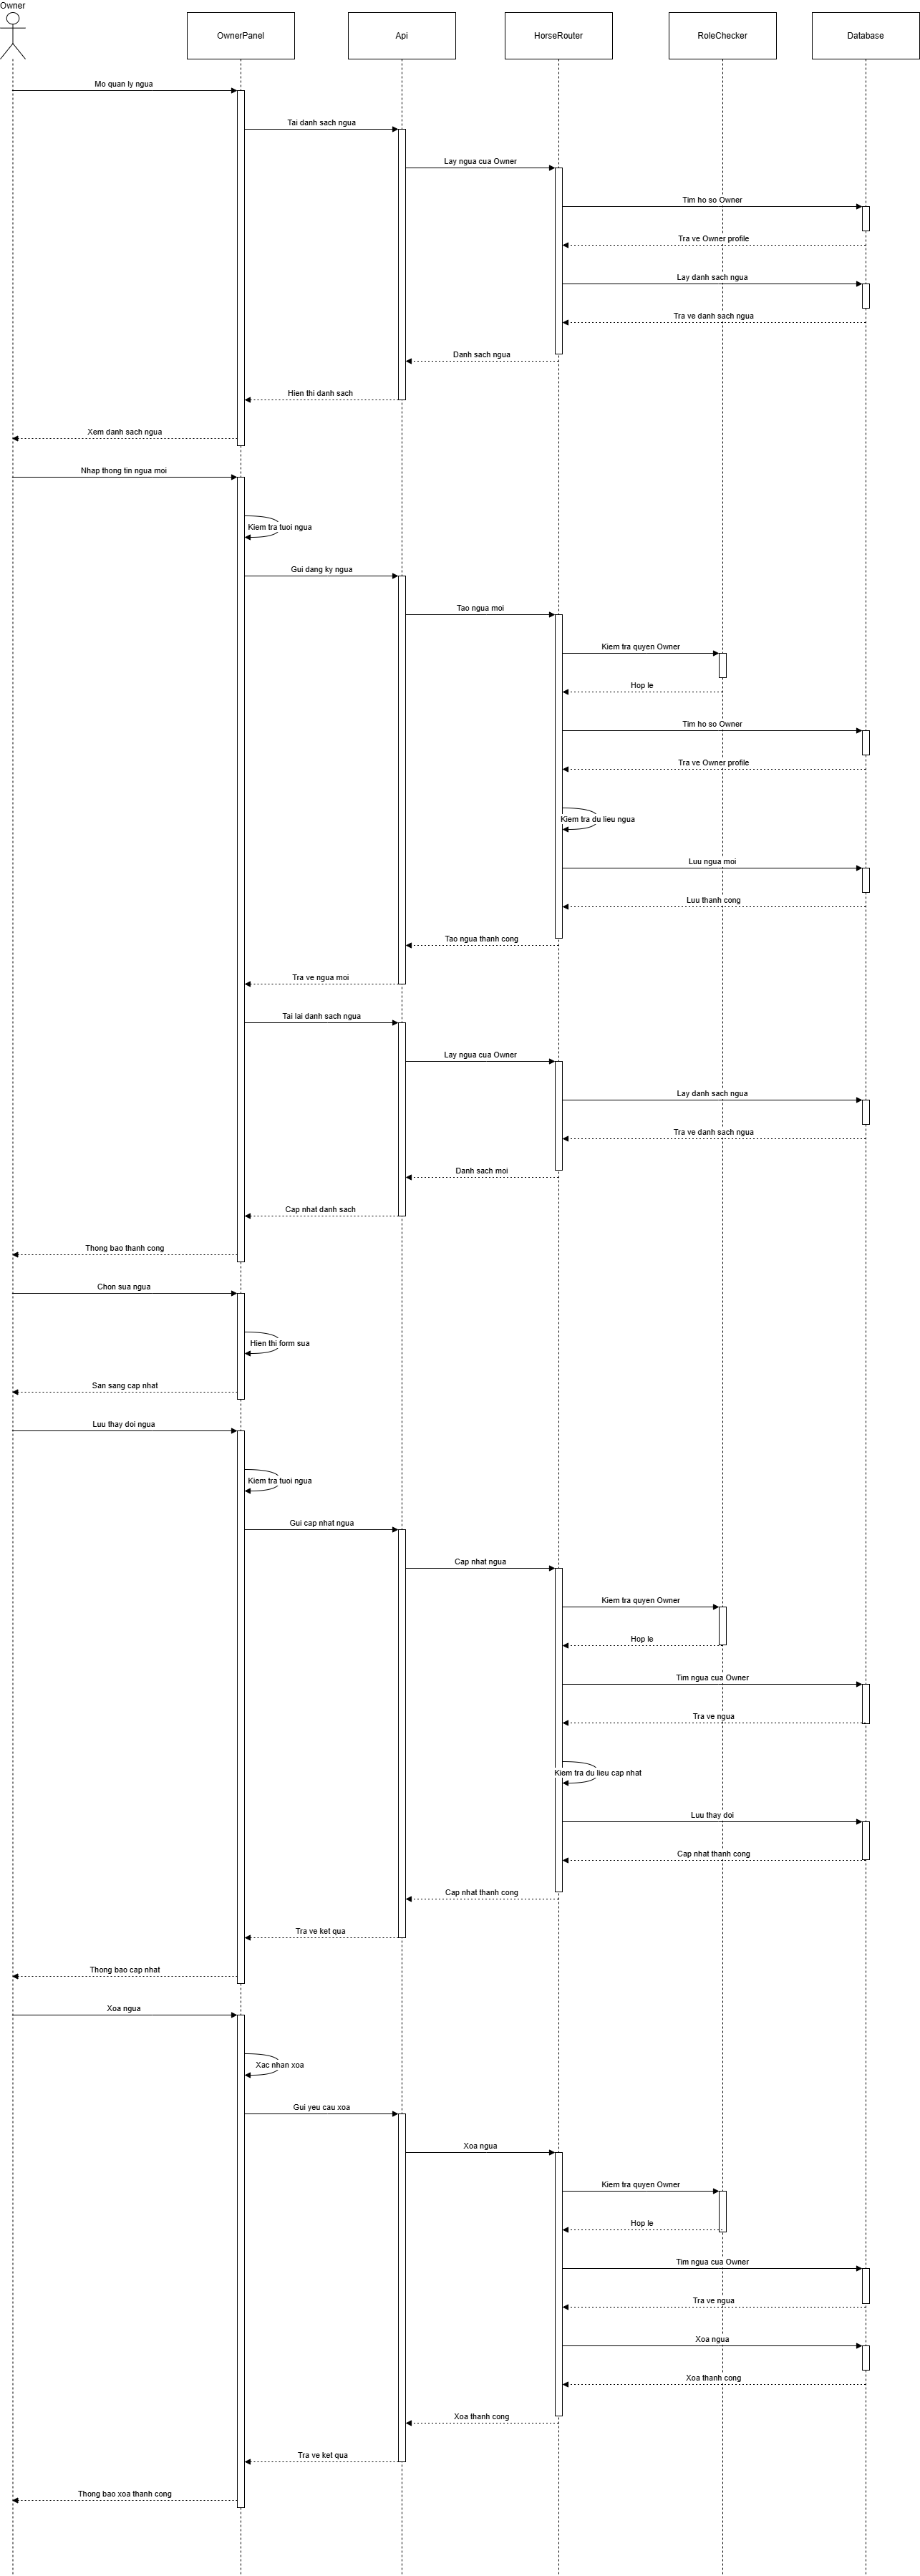
\includegraphics[width=\textwidth,height=0.78\textheight,keepaspectratio]{figures/design/horse_owner/management_sequence.png}
    \caption{Horse Owner Management Operations Sequence Diagram}
    \label{fig:horse_owner_management_sequence_diagram}
\end{figure}

\subsubsection{Class Specification}

\begingroup
\small
\setlength{\tabcolsep}{3pt}
\begin{longtable}{|>{\raggedright\arraybackslash}p{0.16\textwidth}|>{\raggedright\arraybackslash}p{0.30\textwidth}|>{\raggedright\arraybackslash}p{0.14\textwidth}|>{\raggedright\arraybackslash}p{0.25\textwidth}|}
\caption{Horse Owner management operations class specification}
\label{tab:horse_owner_management_class_spec} \\
\hline
\tableHeader
\textbf{Class} & \textbf{Attributes / Methods} & \textbf{Type} & \textbf{Description} \\
\hline
\endfirsthead
\hline
\tableHeader
\textbf{Class} & \textbf{Attributes / Methods} & \textbf{Type} & \textbf{Description} \\
\hline
\endhead
Owner\allowbreak{}Dashboard & activeTab, openHorseManagement() & boundary / UI & Provides the owner dashboard navigation and opens the horse management tab for owner operations. \\
\hline
Owner\allowbreak{}Panel & horses, newHorse, editingHorse, editHorseForm, loadData(), createHorse(), startEditHorse(), updateHorse(), deleteHorse(), cancelEdit() & boundary / UI & Displays the list of owned horses and manages the create, update, and delete interactions from the frontend. \\
\hline
Api & baseUrl, token, get(), post(), put(), delete(), getHeaders() & service / helper & Sends horse management requests to the backend and attaches the owner authentication token to protected API calls. \\
\hline
Horse\allowbreak{}Router & read\_horses(), create\_horse(), update\_horse(), delete\_horse() & controller / route & Handles HTTP requests for viewing, registering, editing, and deleting horses owned by the authenticated owner. \\
\hline
Role\allowbreak{}Checker & allowed\_roles, \_\_call\_\_() & service / authorization & Verifies that the current authenticated user has the \texttt{OWNER} role before allowing protected horse operations. \\
\hline
Horse\allowbreak{}Create & name, age, breed, gender & DTO / request & Carries the input data required to register a new horse; age must be between 2 and 10. \\
\hline
Horse\allowbreak{}Update & name, age, breed, gender & DTO / request & Carries optional horse fields submitted when an owner edits an existing horse record. \\
\hline
Horse\allowbreak{}Out & id, name, age, breed, gender, owner\_id & DTO / response & Returns horse information to the frontend after list, create, or update operations. \\
\hline
User & id, username, email, full\_name, role\_id, is\_active & entity & Represents the authenticated account used to identify the owner performing horse management operations. \\
\hline
Role & id, name & entity & Defines the user's role and supports authorization checks for owner-only operations. \\
\hline
HorseOwner\allowbreak{}Profile & id, user\_id, company\_name, horses & entity & Stores owner-specific information and links the authenticated owner to the horses they manage. \\
\hline
Horse & id, name, age, breed, gender, owner\_id & entity & Database entity storing horse records owned and managed by a horse owner. \\
\hline
\end{longtable}
\endgroup

\subsection{Send Jockey Invitation}
\subsubsection{Class Diagram}

\begin{figure}[H]
    \centering
    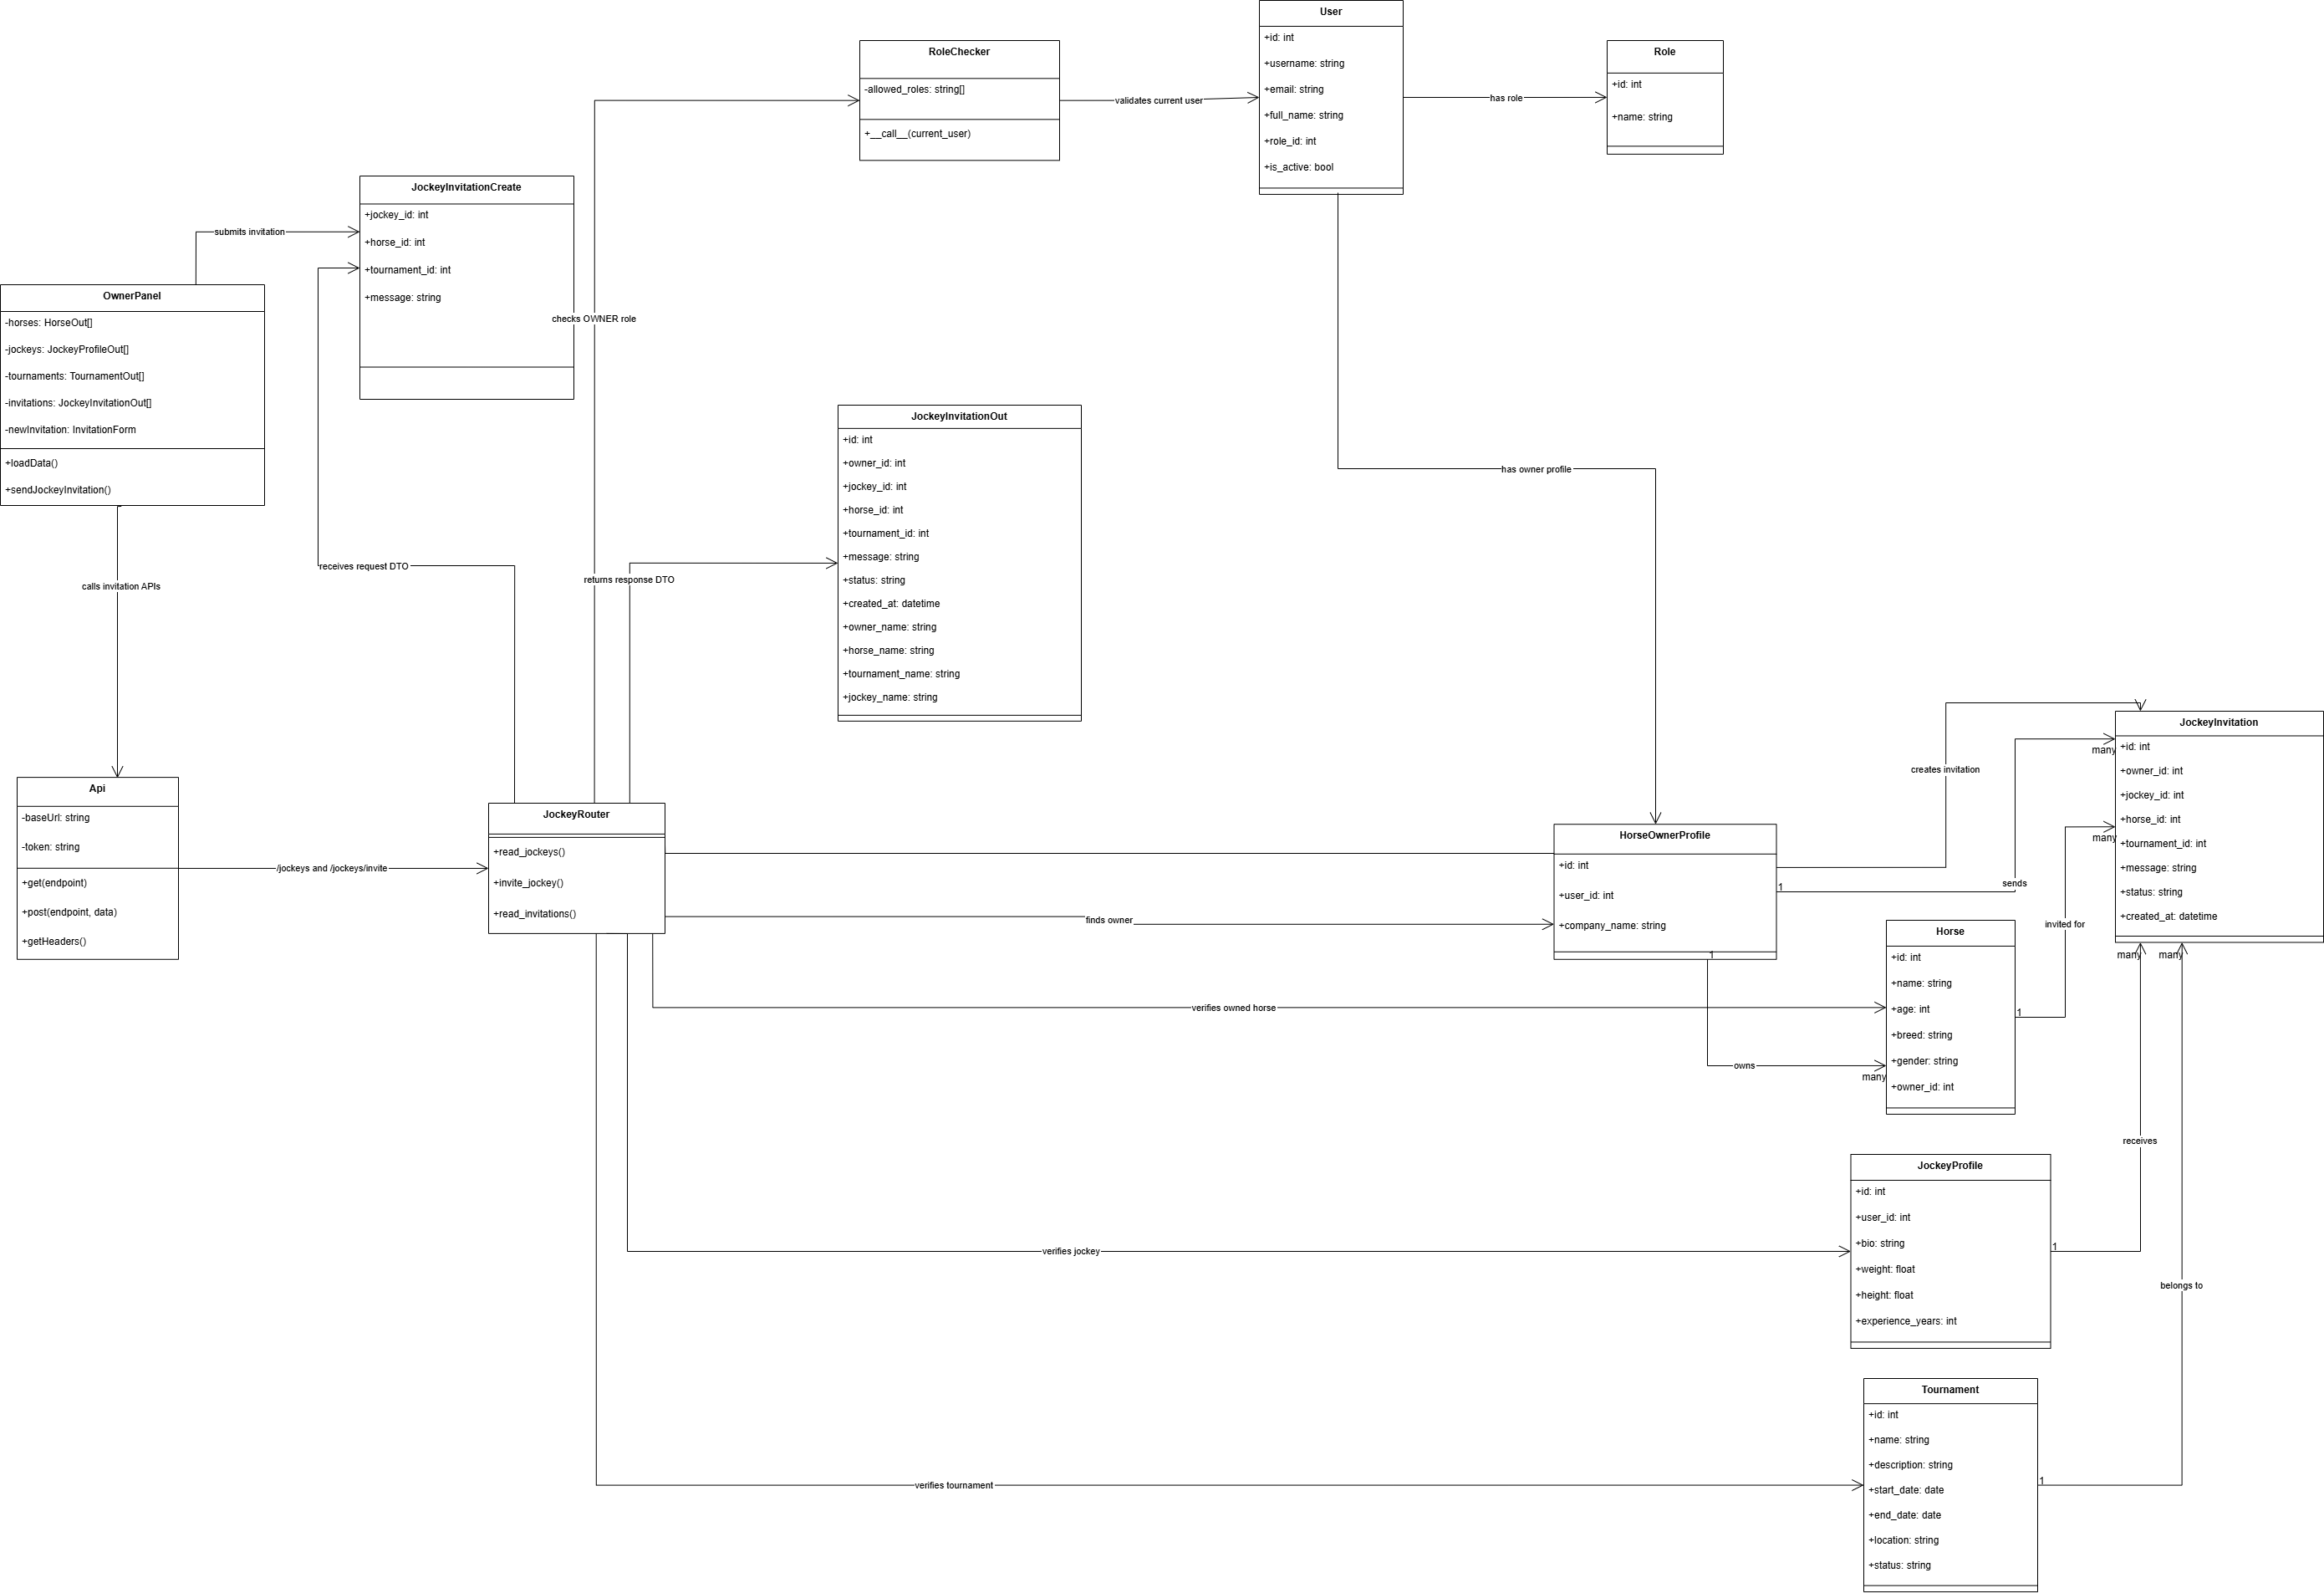
\includegraphics[width=\textwidth,height=0.78\textheight,keepaspectratio]{figures/design/horse_owner/jockey_invication_class.png}
    \caption{Send Jockey Invitation Class Diagram}
    \label{fig:horse_owner_jockey_invitation_class_diagram}
\end{figure}

\subsubsection{Sequence Diagram}

\begin{figure}[H]
    \centering
    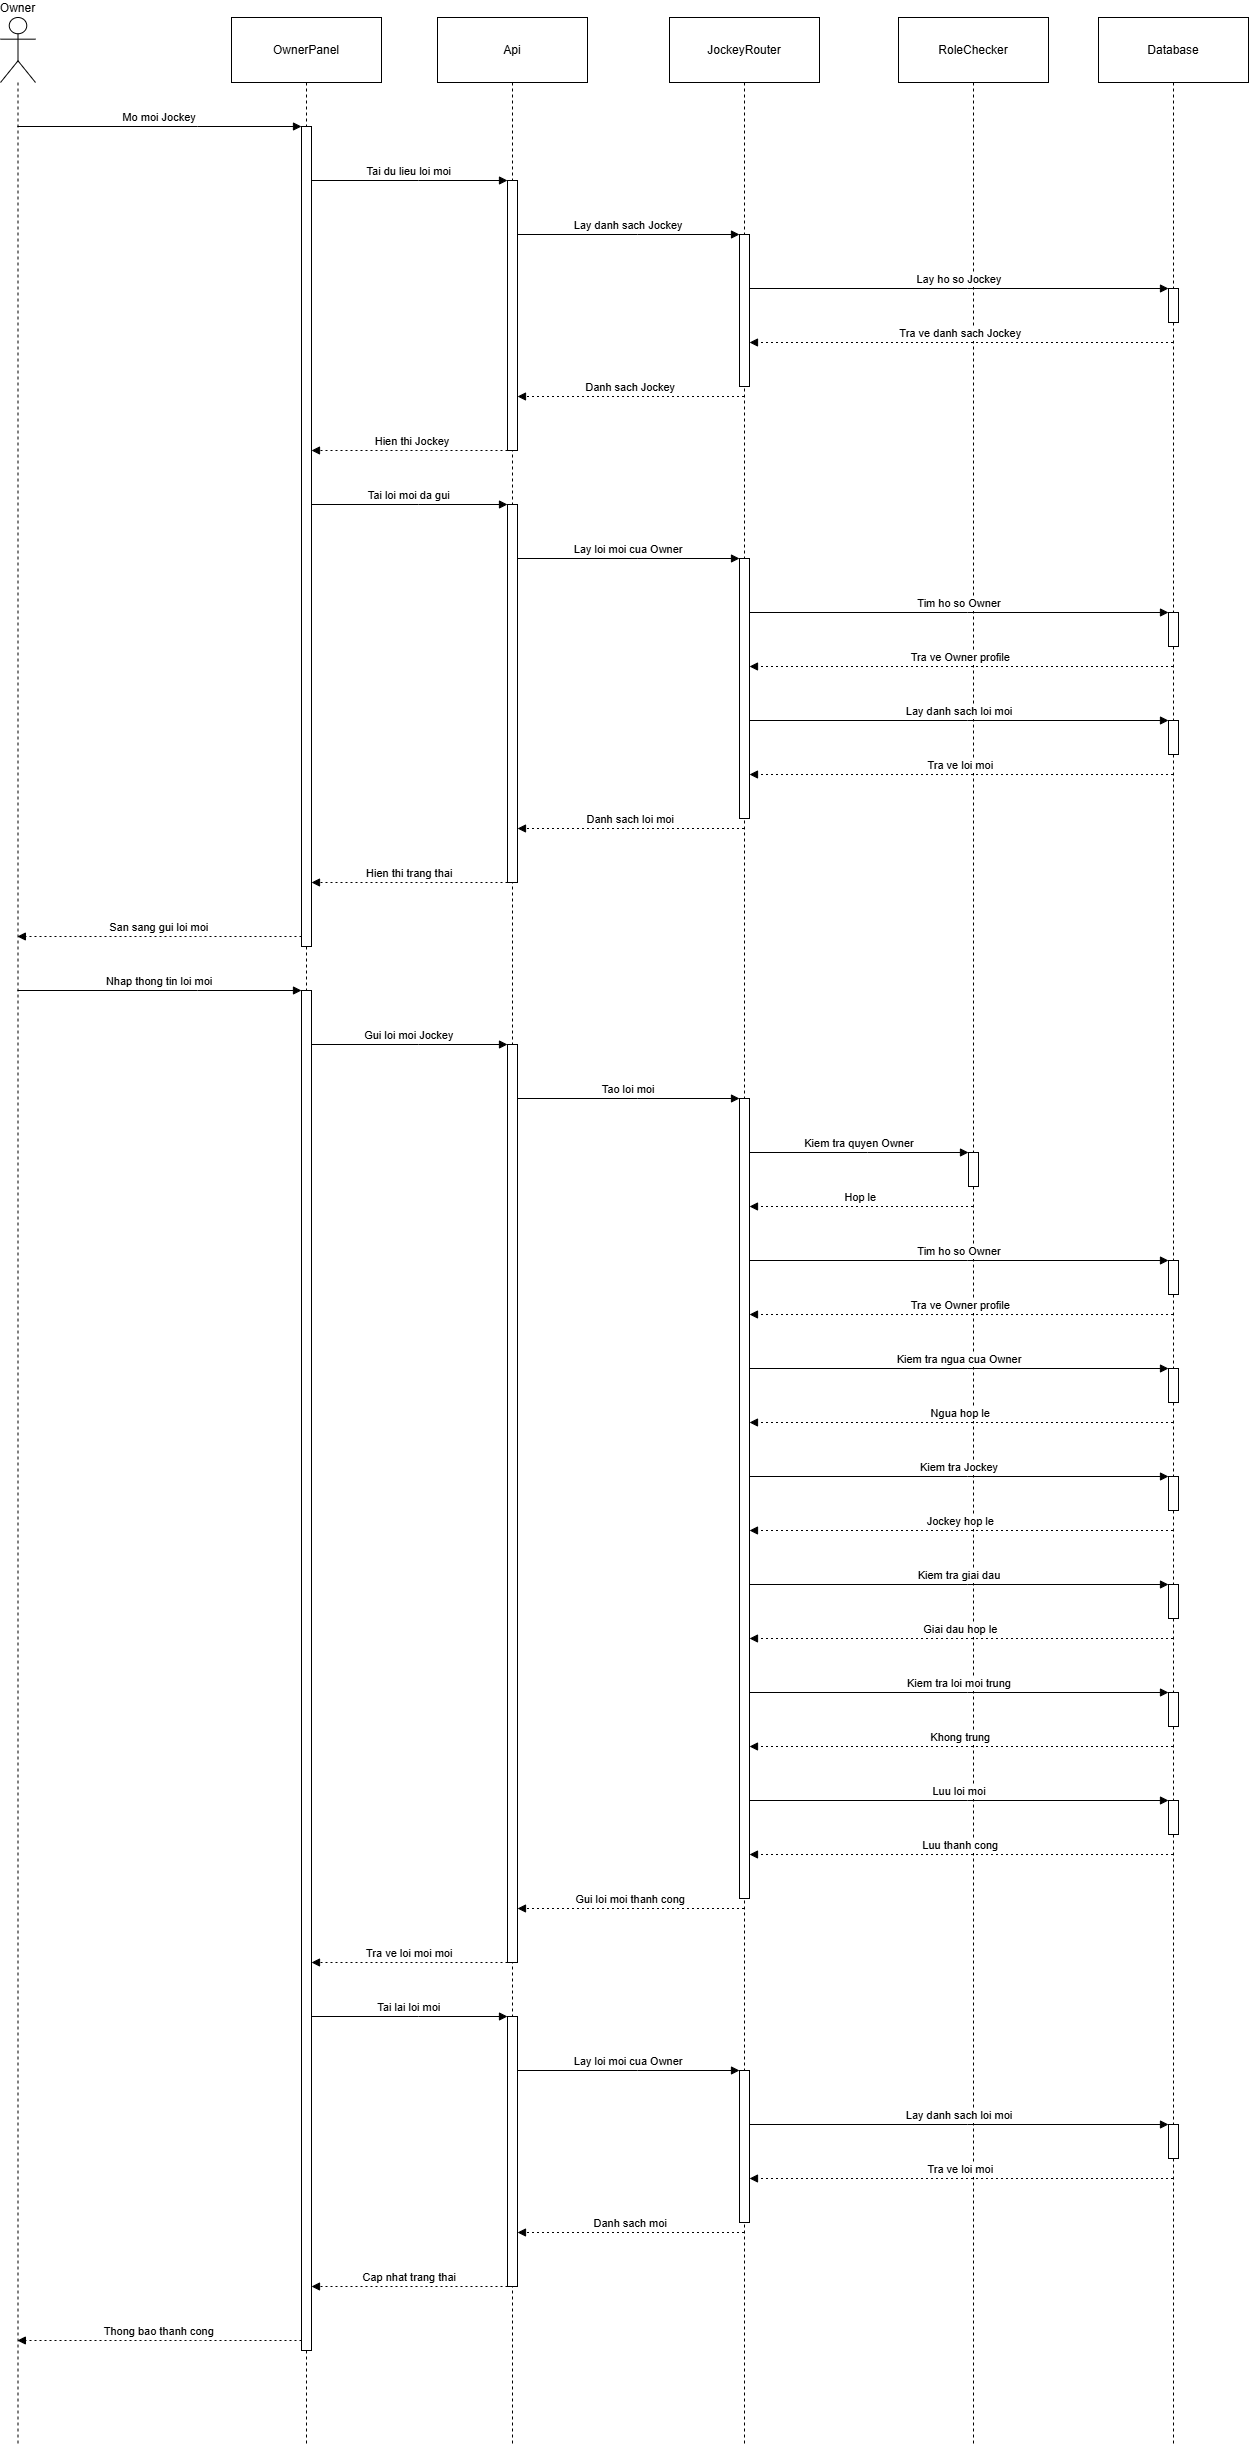
\includegraphics[width=\textwidth,height=0.78\textheight,keepaspectratio]{figures/design/horse_owner/jockey_invitation_sequence.png}
    \caption{Send Jockey Invitation Sequence Diagram}
    \label{fig:horse_owner_jockey_invitation_sequence_diagram}
\end{figure}

\subsubsection{Class Specification}
\begingroup
\small
\setlength{\tabcolsep}{3pt}
\begin{longtable}{|>{\raggedright\arraybackslash}p{0.16\textwidth}|>{\raggedright\arraybackslash}p{0.30\textwidth}|>{\raggedright\arraybackslash}p{0.14\textwidth}|>{\raggedright\arraybackslash}p{0.25\textwidth}|}
\caption{Send Jockey Invitation class specification}
\label{tab:horse_owner_jockey_invitation_class_spec} \\
\hline
\tableHeader
\textbf{Class} & \textbf{Attributes / Methods} & \textbf{Type} & \textbf{Description} \\
\hline
\endfirsthead
\hline
\tableHeader
\textbf{Class} & \textbf{Attributes / Methods} & \textbf{Type} & \textbf{Description} \\
\hline
\endhead
Owner\allowbreak{}Panel & horses, jockeys, tournaments, invitations, newInvitation, loadData(), sendJockeyInvitation() & boundary / UI & Displays the invitation form, loads available horses, jockeys, tournaments, and shows the status of invitations already sent by the owner. \\
\hline
Api & baseUrl, token, get(), post(), getHeaders() & service / helper & Sends requests to retrieve jockeys and invitations, and submits new invitation data to the backend with authorization headers. \\
\hline
Jockey\allowbreak{}Router & read\_jockeys(), invite\_jockey(), read\_invitations() & controller / route & Handles HTTP requests for listing jockey profiles, creating owner invitations, and retrieving invitation status records. \\
\hline
Role\allowbreak{}Checker & allowed\_roles, \_\_call\_\_() & service / authorization & Ensures that only an authenticated user with the \texttt{OWNER} role can send a jockey invitation. \\
\hline
JockeyInvitation\allowbreak{}Create & jockey\_id, horse\_id, tournament\_id, message & DTO / request & Carries the selected jockey, horse, tournament, and optional invitation message submitted by the owner. \\
\hline
JockeyInvitation\allowbreak{}Out & id, owner\_id, jockey\_id, horse\_id, tournament\_id, message, status, created\_at, owner\_name, horse\_name, tournament\_name, jockey\_name & DTO / response & Returns the created or retrieved invitation information, including related display names and current invitation status. \\
\hline
User & id, username, email, full\_name, role\_id, is\_active & entity & Represents the authenticated account used to identify the owner and resolve jockey display information. \\
\hline
Role & id, name & entity & Defines user roles and supports owner-only authorization for sending invitations. \\
\hline
HorseOwner\allowbreak{}Profile & id, user\_id, company\_name & entity & Stores owner-specific information and links the authenticated owner to the invitations they send. \\
\hline
Horse & id, name, age, breed, gender, owner\_id & entity & Represents the horse selected by the owner and is validated to ensure it belongs to the current owner. \\
\hline
Jockey\allowbreak{}Profile & id, user\_id, bio, weight, height, experience\_years & entity & Represents the jockey profile selected as the invitation recipient. \\
\hline
Tournament & id, name, description, start\_date, end\_date, location, status & entity & Represents the tournament context in which the owner invites a jockey to partner with a horse. \\
\hline
Jockey\allowbreak{}Invitation & id, owner\_id, jockey\_id, horse\_id, tournament\_id, message, status, created\_at & entity & Stores the invitation record and tracks whether it is \texttt{PENDING}, \texttt{ACCEPTED}, or \texttt{REJECTED}. \\
\hline
\end{longtable}
\endgroup
